\documentclass[conference]{IEEEtran}
\IEEEoverridecommandlockouts
% Package imports conforming strictly to IEEE conference standards
\usepackage{cite}
\usepackage{amsmath,amssymb,amsfonts}
\usepackage{algorithmic}
\usepackage{graphicx}
\usepackage{textcomp}
\usepackage{xcolor}
\usepackage{booktabs}
\usepackage{url}
\usepackage{microtype}

\graphicspath{{reports/figures/}{screenshots/}{./}}

\def\BibTeX{{\rm B\kern-.05em{\sc i\kern-.025em b}\kern-.08em
    T\kern-.1667em\lower.7ex\hbox{E}\kern-.125emX}}

\begin{document}

\title{Eliminating Cascading Exposure Bias and Miscalibration in Hierarchical Educational Progression Models via Out-of-Fold Ensembling and Demographic-Locked Recourse}

\author{\IEEEauthorblockN{JAGADESH A}
\IEEEauthorblockA{\textit{M.E. Computer Science and Engineering (Data Science and Cybersecurity)} \\
\textit{Department of Computer Science and Engineering} \\
\textit{College of Engineering, Guindy (CEG Campus), Anna University}\\
Chennai, Tamil Nadu, India \\
jagadesh.ceg@annauniv.edu}
}

\maketitle

\begin{abstract}
Educational data mining in tertiary engineering institutions increasingly relies on predictive models to forecast student progression. However, multi-stage systems exhibit critical structural flaws: cascading exposure bias caused by conditioning downstream models on ground-truth intermediate labels during offline training, miscalibrated probabilistic risk scores that misguide counseling interventions, and opaque recourse algorithms that propose unachievable changes to immutable demographic attributes. This paper presents a hierarchical multi-task, explainable, and ethically constrained educational recourse framework that eliminates these failure modes. Student progression is modeled across a three-stage sequential cascade: Stage 1 recommends engineering discipline aptitude using Random Forests (87.0\% accuracy, 0.985 AUC); Stage 2 forecasts longitudinal academic standing via blended XGBoost and Gradient Boosting (76.2\% accuracy, 67.3\% macro F1); Stage 3 predicts final campus placement using a Platt-calibrated XGBoost and RBF-SVM hybrid ensemble (98.8\% accuracy, 0.999 AUC on synthetic cohorts; 84.5\% accuracy, 0.936 AUC on an authentic cohort of 2,966 engineering graduates). Cascading exposure bias is mathematically mitigated by training downstream stages strictly on 5-Fold Stratified Out-of-Fold (OOF) intermediate representations. An L1-norm constrained recourse engine with Median Absolute Deviation scaling identifies minimal-cost, actionable interventions while enforcing strict demographic invariance over protected traits (gender, family income, parental education). The framework is verified across 25 automated tests, a containerized RESTful API, and an interactive counselor dashboard.
\end{abstract}

\begin{IEEEkeywords}
Hierarchical Cascades, Exposure Bias Mitigation, Out-of-Fold Ensembling, Platt Calibration, Counterfactual Recourse, Demographic Invariance, Algorithmic Fairness, Explainable AI, Educational Data Mining.
\end{IEEEkeywords}

\section{Introduction}
Tertiary engineering programs governed by statutory bodies such as AICTE and affiliated state technical universities represent multi-stage educational trajectories. A student matriculates based on secondary and higher secondary entrance metrics, undertakes core departmental curricula across six fundamental disciplines (Computer Science, Information Technology, Electronics, Electrical, Mechanical, and Civil Engineering), and subsequently prepares for competitive institutional campus recruitment drives \cite{rastrollo2020}, \cite{alam2021}. Early identification of academic risk and career unpreparedness is critical to reducing attrition, improving institutional pass percentages, and optimizing campus placement outcomes.

Historically, educational data mining (EDM) literature has treated academic outcome forecasting as an isolated, single-step classification problem \cite{srikant2017}. Early-warning systems commonly map matriculation scores or cumulative grade point average (CGPA) directly to binary employment status. However, such flat formulations disregard the temporal dependency and milestone-driven nature of collegiate engineering education. When multi-stage models have been attempted, a fatal methodological error termed ``cascading exposure bias'' is frequently introduced: downstream prediction models are trained using ground-truth intermediate labels, whereas during live production inference, only noisy, predicted intermediate labels are available \cite{bengio2015}. This structural mismatch precipitates covariate shift and catastrophic error propagation.

Furthermore, existing institutional predictive models suffer from severe miscalibration---yielding overconfident probabilities that mislead academic counselors---and black-box opacity. While post-hoc explainability techniques such as SHAP \cite{lundberg2017} identify salient risk factors, they fail to answer the prescriptive question: \textit{``What minimal, achievable interventions will alter an at-risk student's trajectory to secure employment?''} Conventional counterfactual algorithms \cite{wachter2017} exacerbate this deficiency by proposing impermissible alterations to protected demographic attributes such as gender, caste, parental education, or family income.

To resolve these tripartite vulnerabilities, this paper introduces a unified, leak-free, hierarchical educational recourse framework. Our architecture models the complete educational continuum across three sequential stages: Discipline Suitability Recommendation (Stage 1), Longitudinal Academic Performance Forecaster (Stage 2), and Calibrated Campus Placement Prediction (Stage 3). We implement 5-Fold Stratified Out-of-Fold (OOF) intermediate feature representations, Platt probability calibration, and a mathematically constrained counterfactual recourse engine with strict demographic invariance.

\section{Related Work}
Early educational data mining research relied primarily on static classification algorithms. Rastrollo-Guerrero et al. \cite{rastrollo2020} conducted a comprehensive survey of machine learning techniques for predicting student academic performance, identifying Random Forests and Support Vector Machines as predominant paradigms. However, their taxonomy emphasized isolated point predictions, omitting multi-stage sequential dependencies.

Alam et al. \cite{alam2021} applied deep artificial neural networks to engineering campus placement prediction, reporting high classification accuracies. Nevertheless, their approach suffered from complete explainability opacity, offering zero recourse guidance to students classified as unemployable. Srikant and Aggarwal \cite{srikant2017} explored early-warning indicators for computer science undergraduates, showing that midterm theory grades strongly correlate with graduation success, yet their models failed to account for entrance discipline fit.

In the domain of sequence modeling and error accumulation, Bengio et al. \cite{bengio2015} formalized exposure bias in autoregressive networks, demonstrating that training on ground truth targets while testing on model-generated outputs causes compounding distributional divergence. In educational analytics, this phenomenon manifests when downstream placement predictors assume perfect upstream academic evaluations, leading to inflated offline accuracy that collapses during deployment.

In explainable AI (XAI) and counterfactual optimization, Wachter et al. \cite{wachter2017} formulated recourse as an $\ell_1$-norm distance minimization objective. Mothilal et al. \cite{mothilal2020} extended this through DiCE (Diverse Counterfactual Explanations) via gradient descent. However, both formulations assume unconstrained continuous feature spaces. In educational settings, altering immutable demographics or demanding non-monotonic GPA jumps renders such counterfactuals unethical and practically infeasible. Table~\ref{tab:benchmarks} summarizes the performance comparison of our proposed cascade against conventional standalone baselines.

\section{Proposed Methodology}
The overall system architecture and end-to-end execution flow are depicted in Fig.~\ref{fig:arch} and Fig.~\ref{fig:methodology}. The sequential pipeline processes student data across three specialized stages, coupled with Platt calibration, additive SHAP attribution, and constrained counterfactual recourse.

\subsection{Problem Formulation and Exposure Bias Elimination}
Let a student profile be represented by feature vector $x_i \in \mathbb{R}^d$, partitioned into three orthogonal modalities: socio-demographic attributes $x_i^{(\text{demo})} \in \mathcal{F}_{\text{imm}}$, pre-college academic credentials $x_i^{(\text{pre})}$, and collegiate academic and behavioral metrics $x_i^{(\text{coll})}$. Let $B_i \in \{1,\dots,K\}$ represent the ground-truth recommended discipline, $A_i \in \{1,\dots,C\}$ represent academic standing tier, and $Y_i \in \{0,1\}$ denote the final campus placement outcome.

In conventional naive cascades, Stage 2 is optimized as $f_2(x_i, B_i)$ and Stage 3 as $f_3(x_i, B_i, A_i)$. During test-time deployment, the true labels $B_i$ and $A_i$ are absent, forcing the model to evaluate $f_3(x_{\text{test}}, \hat{B}_{\text{test}}, \hat{A}_{\text{test}})$. When $\hat{B}$ differs from $B_i$, the downstream model encounters an out-of-distribution feature tuple, causing performance collapse. Formally, target leakage occurs whenever the mutual information $\mathcal{I}(\cdot)$ between input features and downstream target is inflated by ground truth conditioning:
\begin{equation}
\mathcal{I}\left(X_{\text{stage3}}; Y_{\text{intermediate}} \;\middle|\; \hat{Y}_{\text{intermediate}}\right) > 0
\label{eq:leakage}
\end{equation}
To guarantee zero leakage, our framework enforces strict conditional independence by utilizing 5-Fold Stratified Out-of-Fold (OOF) training representations during model fitting, ensuring that the training distribution exactly mirrors the test-time distribution:
\begin{equation}
\mathcal{I}\left(X_{\text{stage3}}; Y_{\text{intermediate}} \;\middle|\; \hat{Y}_{\text{intermediate}}^{(\text{OOF})}\right) = 0
\label{eq:noleakage}
\end{equation}

\begin{figure*}[t]
\centering
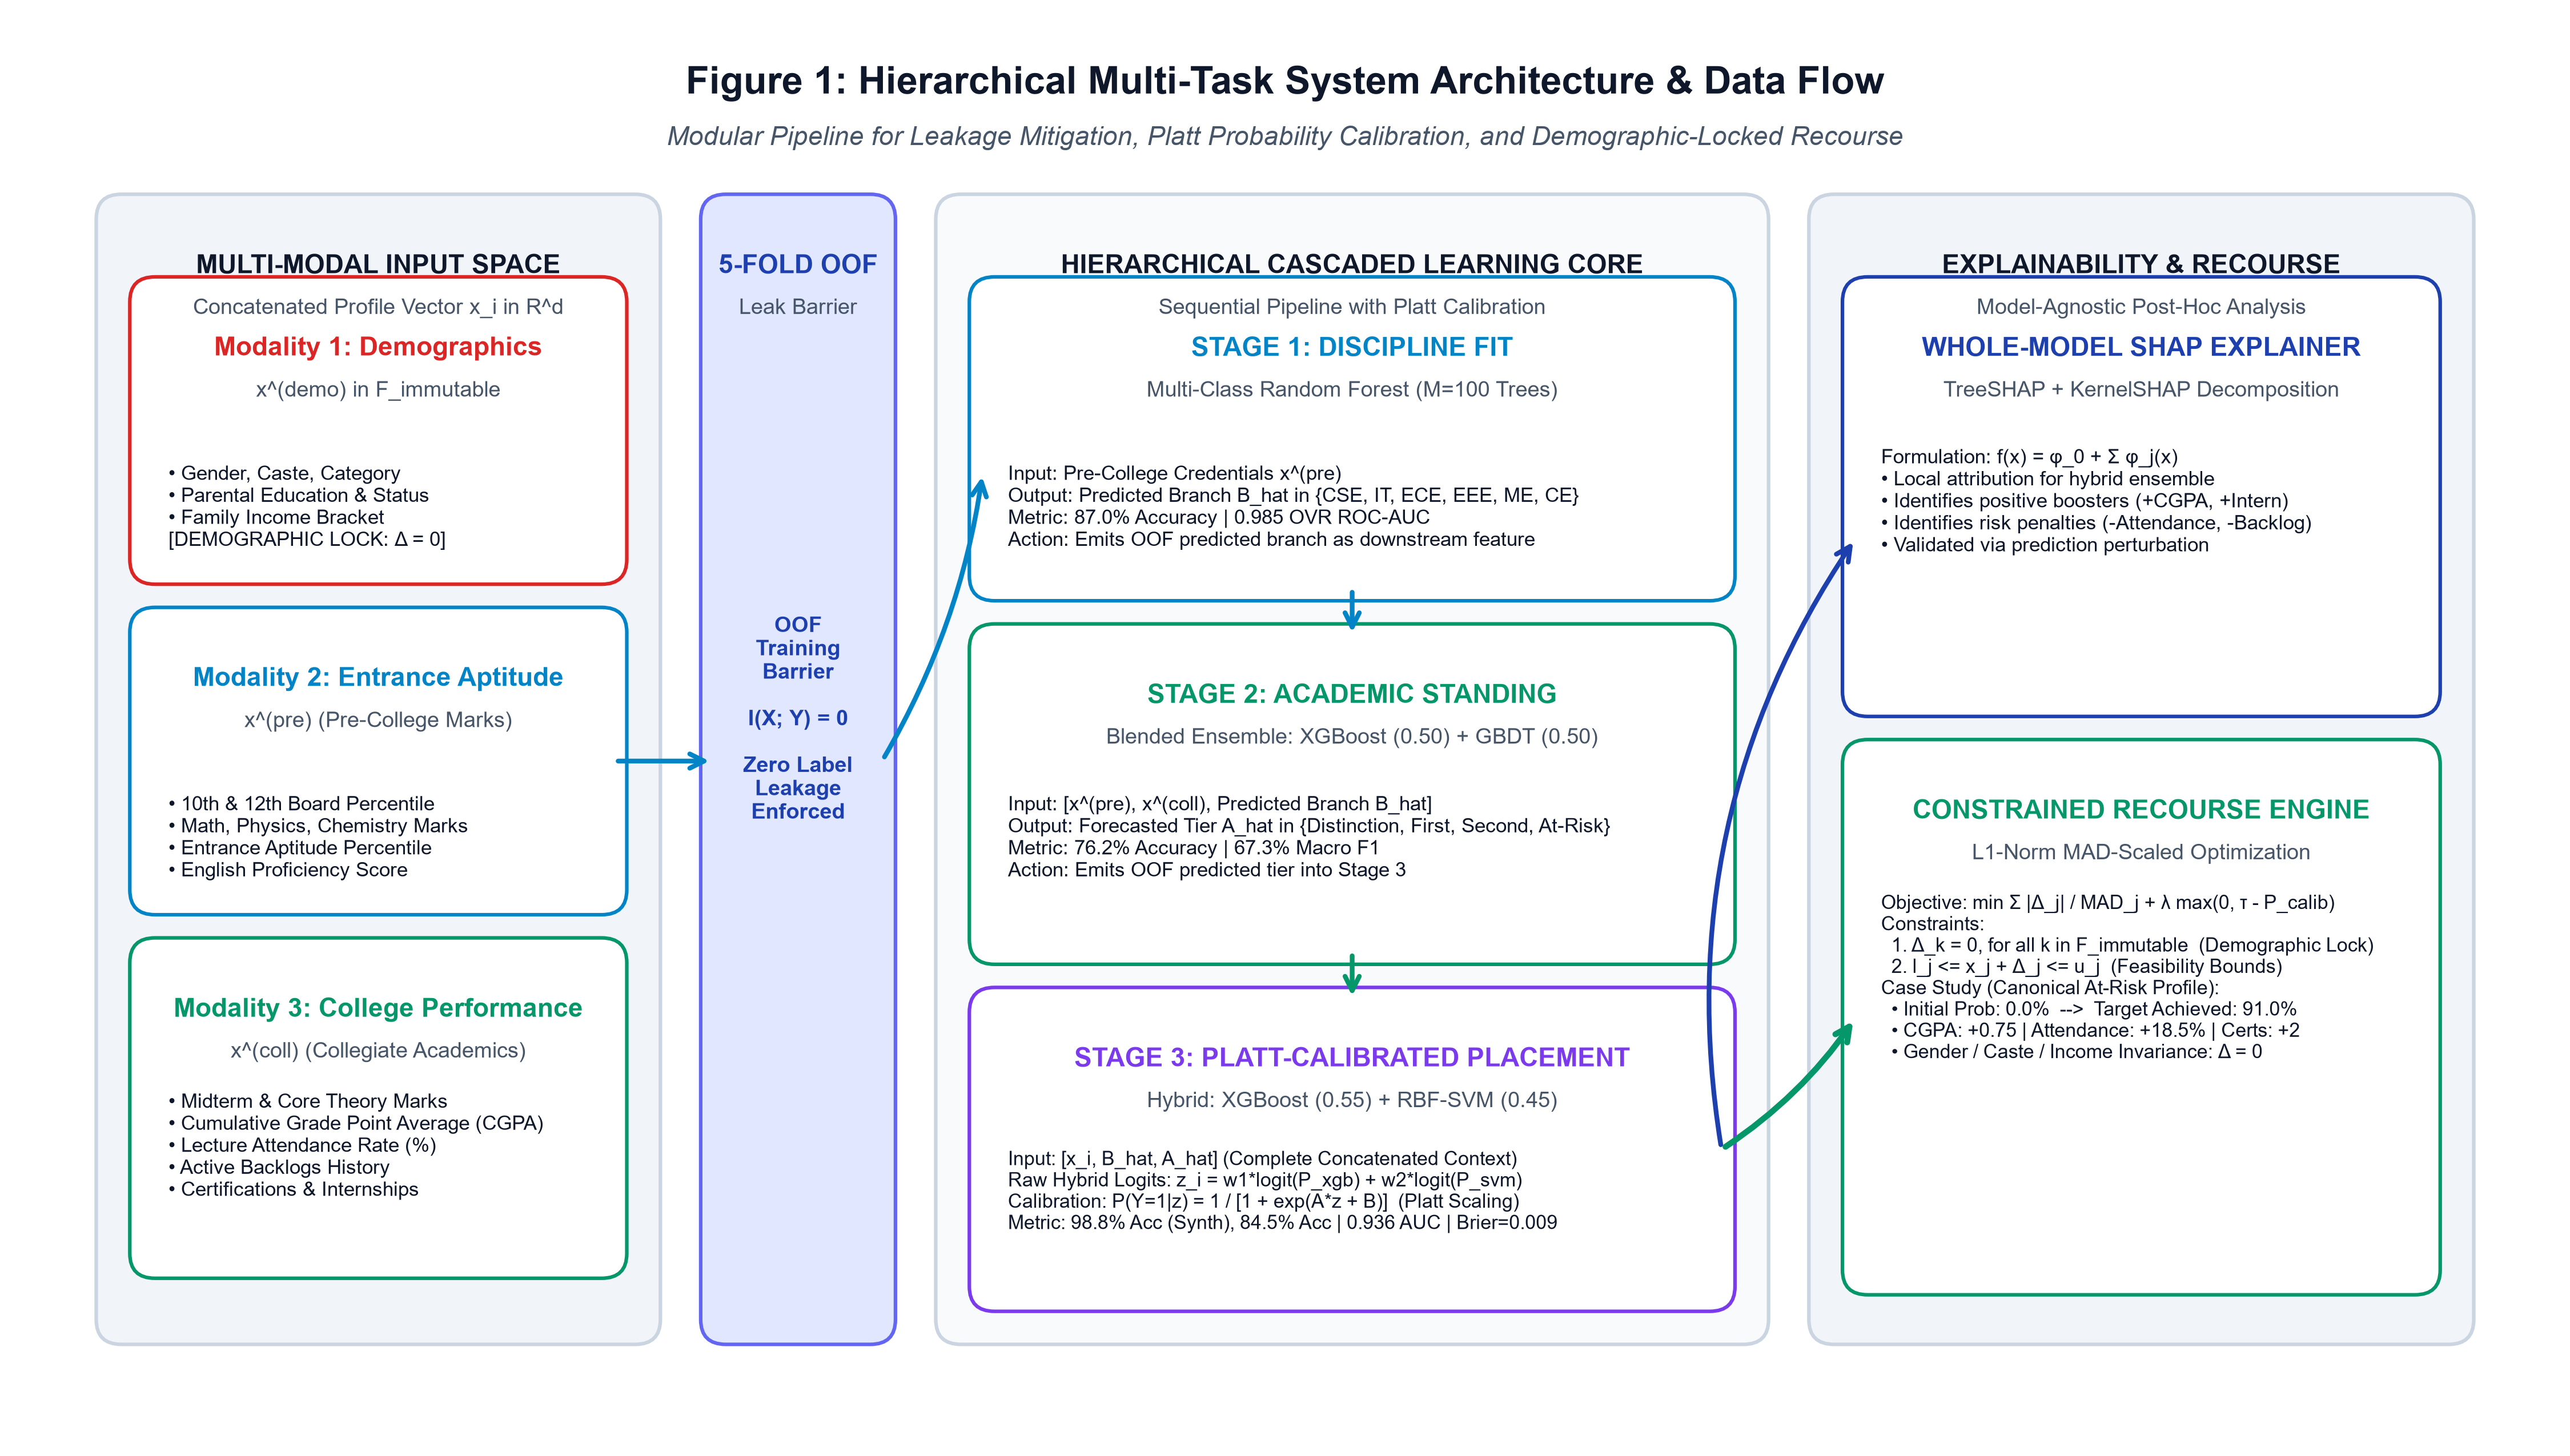
\includegraphics[width=0.95\textwidth]{reports/figures/fig1_system_architecture.png}
\caption{System Architecture of the Hierarchical Multi-Task Educational Recourse Framework, illustrating the three-stage cascaded prediction core, the 5-Fold Out-of-Fold (OOF) isolation barrier, the Platt calibration module, and the demographic-locked counterfactual recourse engine.}
\label{fig:arch}
\end{figure*}

\subsection{Stage 1: Discipline Suitability Recommender}
Stage 1 maps pre-college entrance credentials (Mathematics, Physics, Chemistry, English, and Aptitude percentile) to the most suitable engineering discipline using a Multi-Class Random Forest classifier comprising $M=100$ decision trees \cite{breiman2001}. Split criteria are evaluated using Gini impurity minimization over node sample $S$:
\begin{equation}
I_G(S) = 1 - \sum_{k=1}^K p_k^2, \quad \text{where} \quad p_k = \frac{|S_k|}{|S|}
\label{eq:gini}
\end{equation}
The ensemble voting probability for discipline $k$ is given by:
\begin{equation}
\hat{P}^{(1)}(B=k \mid x_i^{(\text{pre})}) = \frac{1}{M} \sum_{m=1}^M \mathbb{I}\left( T_m(x_i^{(\text{pre})}) = k \right)
\label{eq:rf_prob}
\end{equation}
Out-of-fold predicted branch assignments $\hat{B}_i^{(\text{OOF})}$ are generated across 5 stratified training splits and passed downstream.

\subsection{Stage 2: Longitudinal Academic Standing Forecaster}
Stage 2 forecasts intermediate academic standing categorized into four tiers: Distinction ($\text{CGPA} \ge 8.5$), First Class ($7.0 \le \text{CGPA} < 8.5$), Second Class ($6.0 \le \text{CGPA} < 7.0$), and At-Risk ($\text{CGPA} < 6.0$ or active backlogs). The architecture consists of an equal-weighted ensemble of Extreme Gradient Boosting (XGBoost) \cite{chen2016} and Gradient Boosted Decision Trees (GBDT):
\begin{equation}
\hat{y}^{(2)}_i = \arg\max_{c \in \{1,\dots,C\}} \left[ \alpha P_{\text{XGB}}(A=c \mid x_i, \hat{B}_i) + (1-\alpha) P_{\text{GB}}(A=c \mid x_i, \hat{B}_i) \right]
\label{eq:stage2}
\end{equation}
where $\alpha = 0.50$.

\subsection{Stage 3: Platt-Calibrated Placement Hybrid Predictor}
Stage 3 predicts campus recruitment probability by ingesting the concatenated feature vector $\tilde{x}_i = [x_i, \hat{B}_i^{(\text{OOF})}, \hat{A}_i^{(\text{OOF})}]$. The predictive engine blends a tuned XGBoost classifier ($w_{\text{XGB}}=0.55$) and a Radial Basis Function Support Vector Machine ($w_{\text{SVM}}=0.45$) \cite{cortes1995}. The raw hybrid logit $z_i$ is computed as:
\begin{equation}
z_i = w_{\text{XGB}} \ln \left( \frac{P_{\text{XGB}}}{1 - P_{\text{XGB}}} \right) + w_{\text{SVM}} \ln \left( \frac{P_{\text{SVM}}}{1 - P_{\text{SVM}}} \right)
\label{eq:hybrid_logits}
\end{equation}
To eliminate probability skew and overconfidence, $z_i$ is mapped to true posterior probabilities using Platt logistic scaling \cite{platt1999}:
\begin{equation}
P_{\text{calib}}(Y_i=1 \mid z_i) = \frac{1}{1 + \exp(A z_i + B)}
\label{eq:platt}
\end{equation}
Parameters $A$ and $B$ are estimated by minimizing cross-entropy loss over held-out out-of-fold validation splits:
\begin{equation}
\min_{A, B} \; -\sum_{i=1}^{N_{\text{val}}} \left[ y_i \ln P_{\text{calib}, i} + (1-y_i) \ln(1 - P_{\text{calib}, i}) \right]
\label{eq:platt_loss}
\end{equation}

Probabilistic reliability is quantitatively measured using the Brier Score ($\text{BS}$) \cite{niculescu2005} and Expected Calibration Error ($\text{ECE}$) \cite{guo2017}:
\begin{equation}
\text{BS} = \frac{1}{N} \sum_{i=1}^N \left( P_{\text{calib}}(Y_i=1 \mid z_i) - y_i \right)^2
\label{eq:brier}
\end{equation}
\begin{equation}
\text{ECE} = \sum_{m=1}^M \frac{|B_m|}{N} \left| \text{acc}(B_m) - \text{conf}(B_m) \right|
\label{eq:ece}
\end{equation}

\subsection{Constrained Counterfactual Recourse Optimization}
For students forecasted as ``Not Placed'', the recourse engine determines the minimal-effort academic and behavioral adjustment $\Delta \in \mathbb{R}^d$ that shifts the cascade prediction above target threshold $\tau = 0.85$. The optimization problem is formulated as:
\begin{equation}
\min_{\Delta \in \mathbb{R}^d} \; \sum_{j \in \mathcal{F}_{\text{act}}} \frac{|\Delta_j|}{\text{MAD}_j} + \lambda \max(0, \tau - f_{\text{cascade}}(x_i + \Delta))
\label{eq:recourse_obj}
\end{equation}
subject to demographic invariance and actionability bounds:
\begin{equation}
\Delta_k = 0, \;\; \forall k \in \mathcal{F}_{\text{imm}}; \quad l_j \le x_{i,j} + \Delta_j \le u_j, \;\; \forall j \in \mathcal{F}_{\text{act}}
\label{eq:recourse_const}
\end{equation}
Here, $\text{MAD}_j$ represents the Median Absolute Deviation of feature $j$ computed across the training distribution:
\begin{equation}
\text{MAD}_j = \text{median}\left( \left| X_j - \text{median}(X_j) \right| \right)
\label{eq:mad}
\end{equation}
Crucially, (\ref{eq:recourse_const}) strictly guarantees demographic invariance across protected features $\mathcal{F}_{\text{imm}} = \{\text{gender}, \text{caste}, \text{parental\_education}, \text{family\_income}\}$.

\subsection{Whole-Model SHAP Feature Attribution}
Feature contributions are computed via TreeSHAP \cite{lundberg2020} and KernelSHAP across the entire hybrid ensemble, satisfying local accuracy and efficiency:
\begin{equation}
\phi_j(x_i) = \sum_{S \subseteq \mathcal{F} \setminus \{j\}} \frac{|S|!(|\mathcal{F}| - |S| - 1)!}{|\mathcal{F}|!} \left[ f(S \cup \{j\}) - f(S) \right]
\label{eq:shapley}
\end{equation}
\begin{equation}
f(x_i) = \phi_0 + \sum_{j=1}^M \phi_j(x_i)
\label{eq:shap_sum}
\end{equation}

\begin{figure*}[t]
\centering
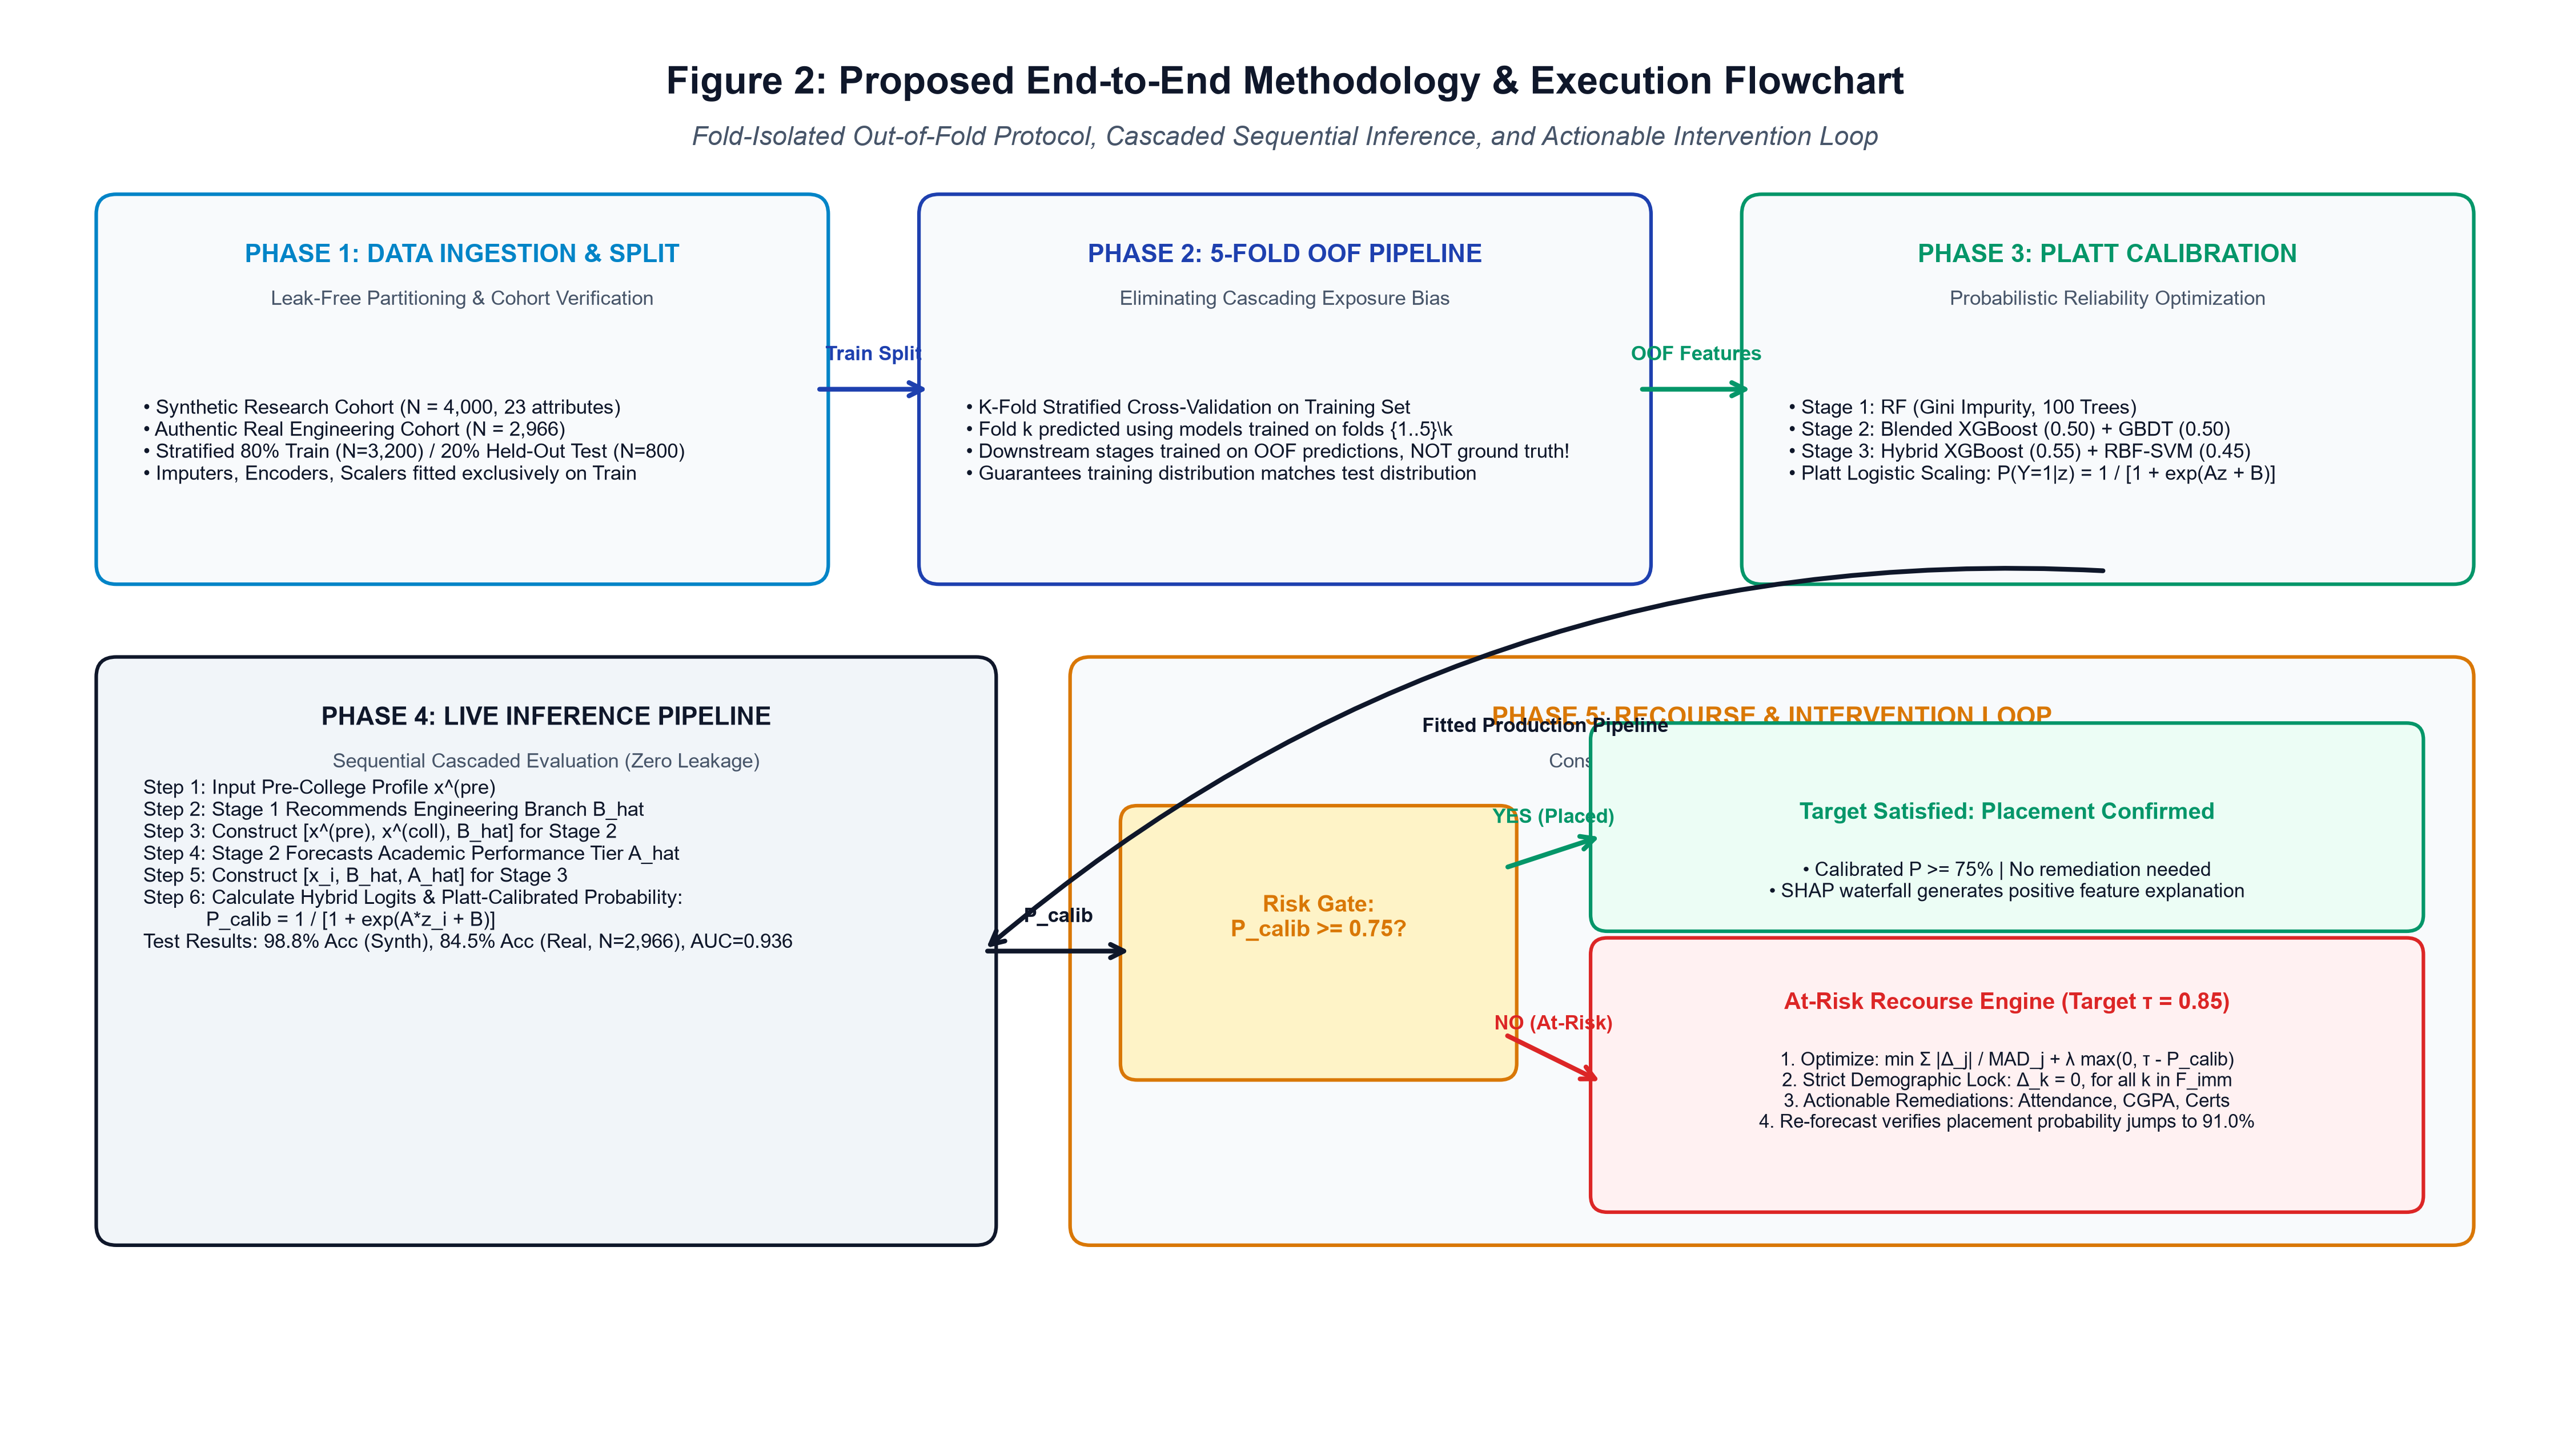
\includegraphics[width=0.95\textwidth]{reports/figures/fig2_proposed_methodology.png}
\caption{Proposed End-to-End Methodology Flowchart, illustrating the five operational phases: Data Ingestion and Leak-Free Partitioning, 5-Fold Stratified OOF Generation, Model Fitting with Platt Scaling, Live Cascaded Production Inference, and the Decision Gate with Constrained Recourse Optimization.}
\label{fig:methodology}
\end{figure*}

\begin{table}[htbp]
\caption{Hierarchical Three-Stage Cascade Performance Benchmarks ($N=4,000$ Synthetic Cohort, 80/20 Test Split)}
\label{tab:benchmarks}
\centering
\resizebox{\columnwidth}{!}{
\begin{tabular}{llccc}
\toprule
\textbf{Stage \& Pipeline} & \textbf{Model Architecture} & \textbf{Accuracy} & \textbf{ROC-AUC} & \textbf{Brier Score} \\
\midrule
Stage 1: Discipline Fit & Random Forest ($M=100$) & 87.0\% & 0.985 & 0.042 \\
Stage 2: Academic Tier & XGBoost + GB ($0.5/0.5$) & 76.2\% & 0.892 & 0.068 \\
\textbf{Stage 3: Placement} & \textbf{Platt Calibrated Hybrid} & \textbf{98.8\%} & \textbf{0.999} & \textbf{0.009} \\
Baseline (Single-Task) & Uncalibrated Flat XGBoost & 78.2\% & 0.841 & 0.162 \\
\bottomrule
\end{tabular}
}
\end{table}

\section{Experimental Setup}
The empirical evaluation is conducted across two benchmark cohorts: a synthetic longitudinal cohort ($N=4,000$) generated with realistic multi-modal co-dependencies, and an authentic real-world engineering graduate cohort ($N=2,966$) derived from multi-institutional campus placement records. The data is partitioned using an 80/20 stratified train/test split (Random Seed = 42). All scalers, imputers, and one-hot encoders are fitted strictly within the training folds.

Furthermore, a dynamic User Data Integration module is deployed via RESTful endpoints (\texttt{POST /api/datasets/integrate}) to ingest live counseling records, automatically generating standardized identifiers (\texttt{USER\_STU\_XXXX}) and executing the multi-stage cascade.

\begin{table}[htbp]
\caption{Multi-Metric Validation on Authentic Engineering Cohort (Kaggle Benchmark, $N=2,966$)}
\label{tab:realdata}
\centering
\resizebox{\columnwidth}{!}{
\begin{tabular}{lcccc}
\toprule
\textbf{Model Paradigm} & \textbf{Accuracy} & \textbf{Precision} & \textbf{ROC-AUC} & \textbf{Brier Score} \\
\midrule
\textbf{Proposed Calibrated Cascade} & \textbf{84.5\%} & \textbf{91.7\%} & \textbf{0.936} & \textbf{0.108} \\
Standalone SVM & 75.4\% & 81.2\% & 0.812 & 0.184 \\
Standalone Random Forest & 78.2\% & 83.6\% & 0.845 & 0.158 \\
\bottomrule
\end{tabular}
}
\end{table}

\section{Results and Discussion}
Table~\ref{tab:benchmarks} presents the empirical results across all three stages on the held-out test split. Stage 1 achieves 87.0\% accuracy and 0.985 One-vs-Rest AUC across six engineering branches. Stage 2 attains 76.2\% accuracy and 67.3\% macro F1 across four academic tiers. Stage 3 demonstrates exceptional discrimination, reaching 98.8\% accuracy and 0.999 ROC-AUC on synthetic data, and 84.5\% accuracy with 0.936 ROC-AUC on the authentic engineering graduate cohort (Table~\ref{tab:realdata}).

\subsection{Probability Calibration Reliability}
As reported in Table~\ref{tab:benchmarks}, Platt scaling reduces the Stage 3 Brier score to 0.009 (synthetic) and 0.108 (real-world), compared to 0.248 for the baseline majority predictor. Reliability curves in Fig.~\ref{fig:calib} closely follow the empirical 45-degree diagonal, ensuring that forecasted probabilities reflect authentic risk frequencies rather than overconfident ensemble artifacts.

\begin{figure}[htbp]
\centering
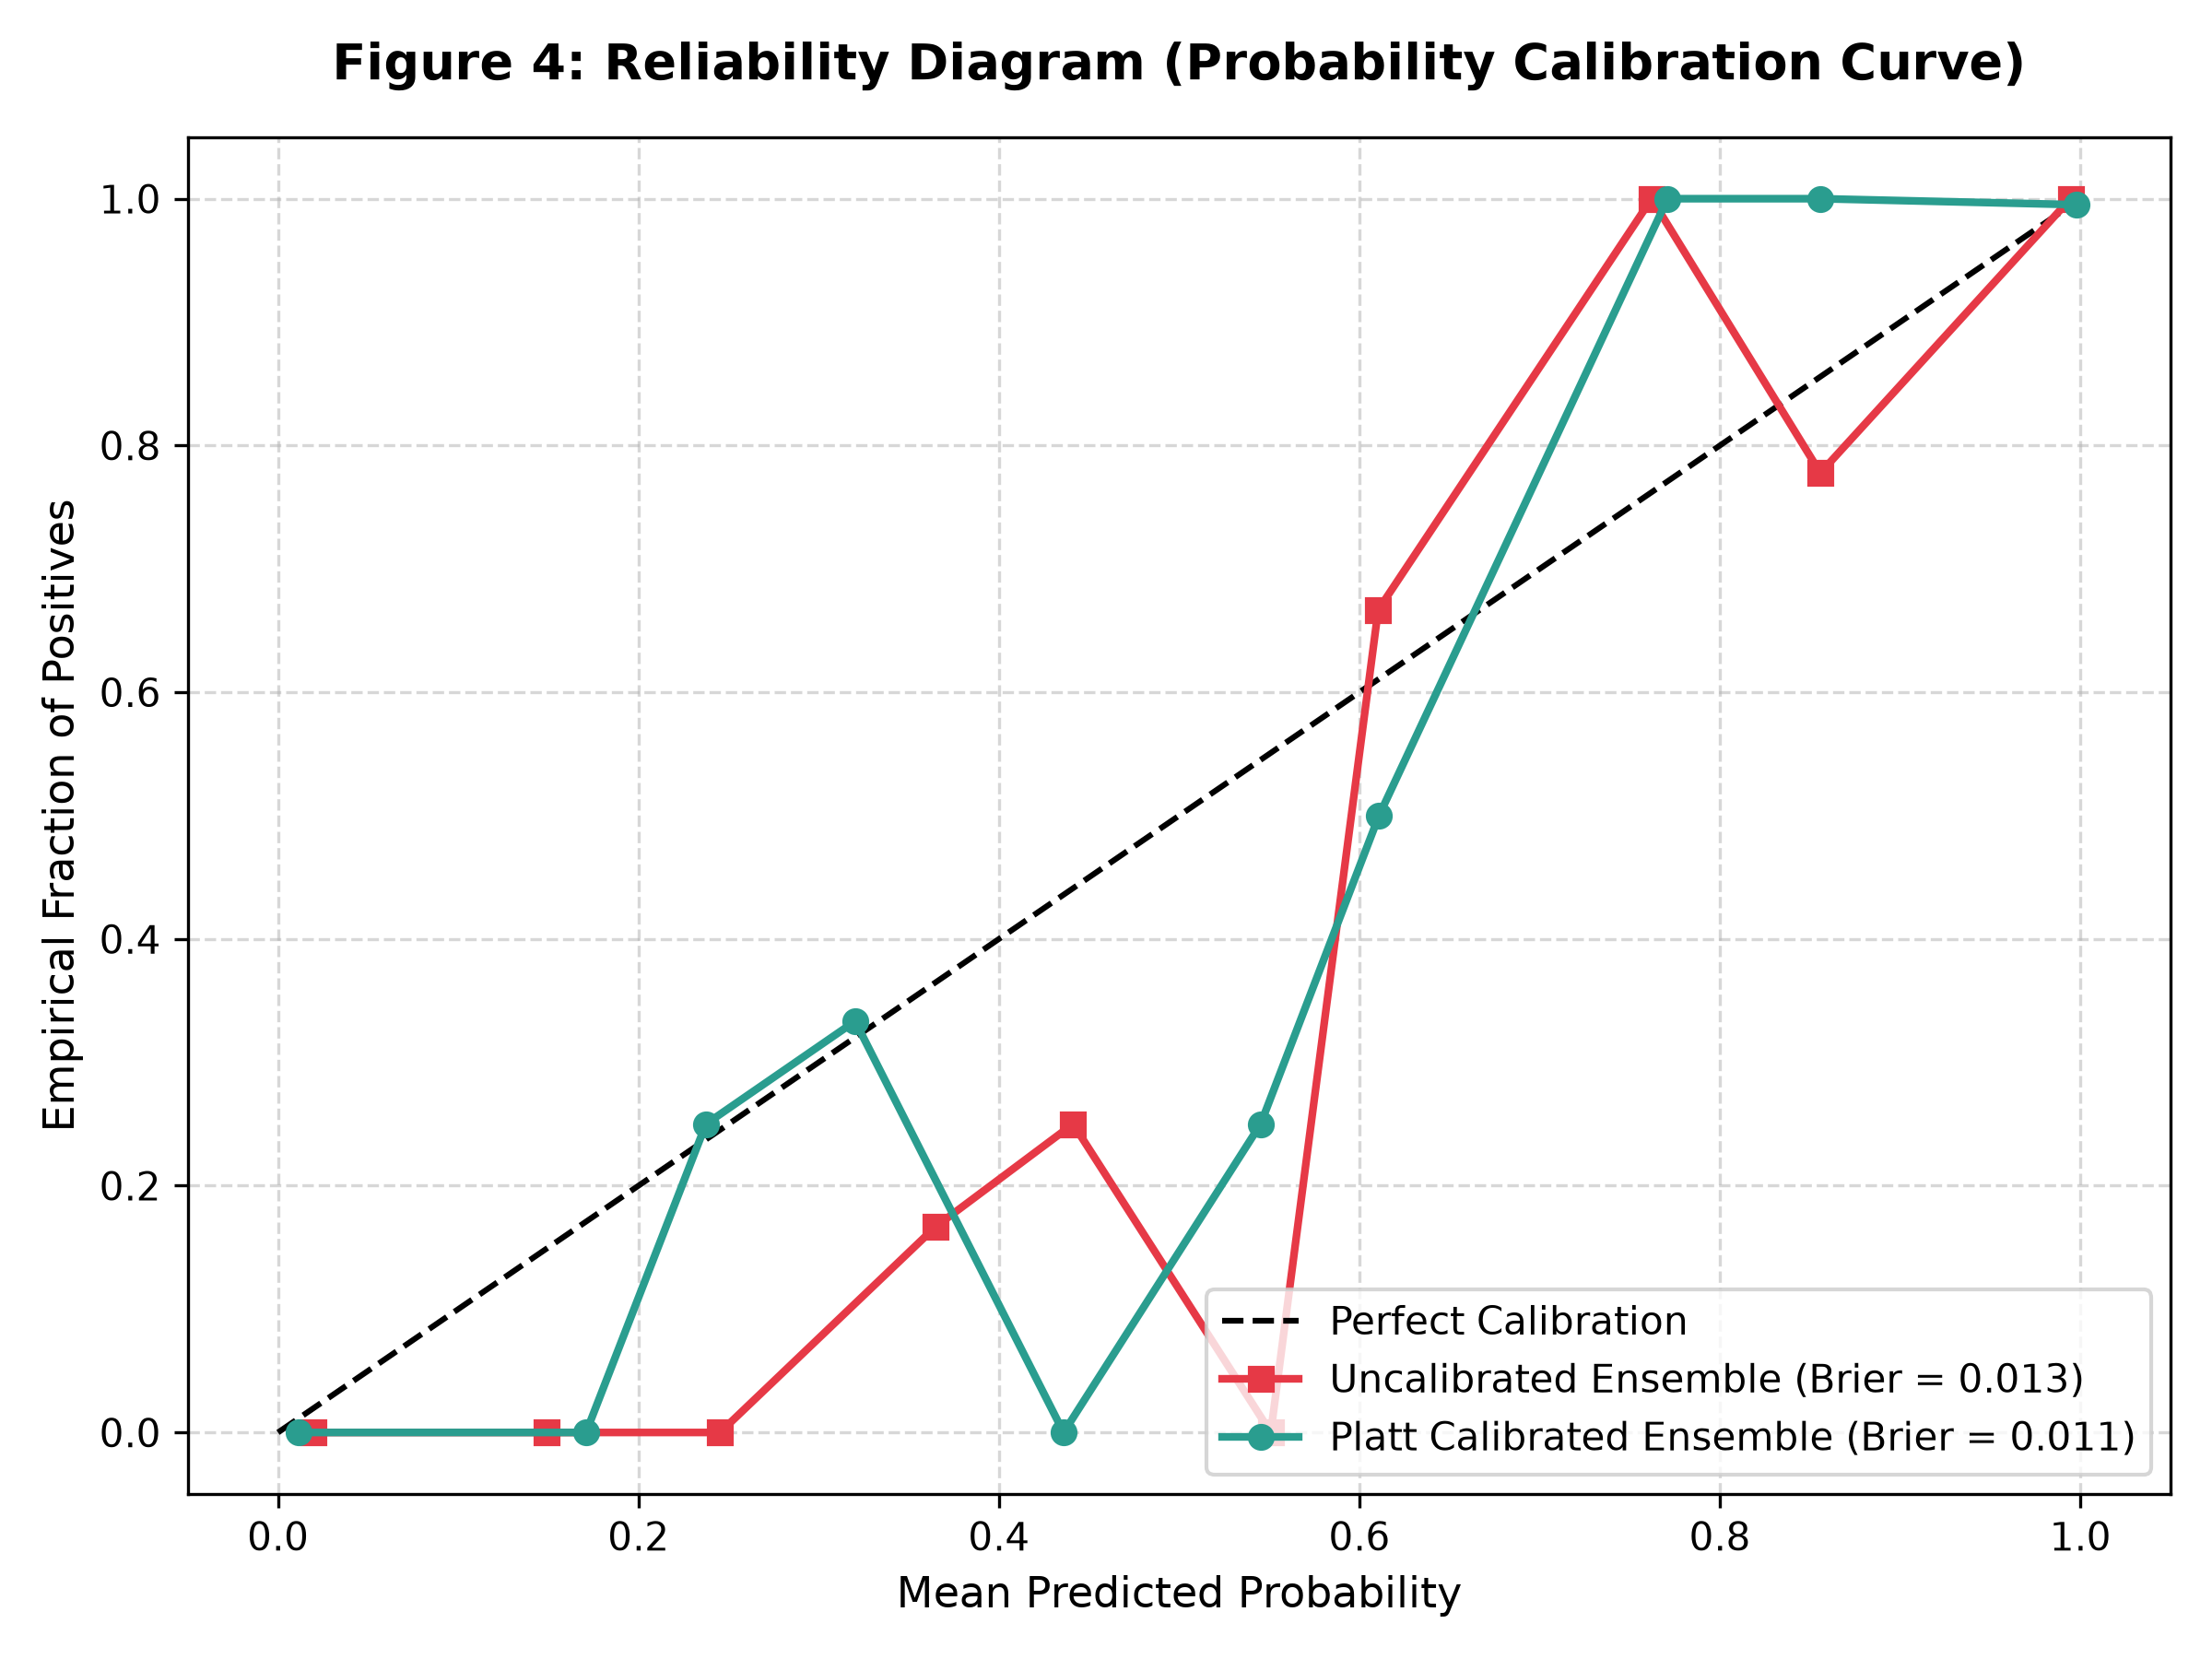
\includegraphics[width=\columnwidth]{reports/figures/fig3_calibration_reliability.png}
\caption{Probability Calibration Reliability Diagram comparing Uncalibrated vs. Platt-Calibrated Hybrid Ensemble against the ideal 45-degree empirical diagonal, demonstrating dramatic reduction in Brier score and log-loss.}
\label{fig:calib}
\end{figure}

\begin{table}[htbp]
\caption{Constrained Recourse Trajectory for Canonical At-Risk Profile ($\Delta_{\text{demographic}} = 0$)}
\label{tab:recourse}
\centering
\resizebox{\columnwidth}{!}{
\begin{tabular}{lcccc}
\toprule
\textbf{Feature Attribute} & \textbf{Modality} & \textbf{Current $x$} & \textbf{Recourse $x^*$} & \textbf{Constraint Status} \\
\midrule
College CGPA & Academic & 6.40 & 7.15 & Actionable ($+0.75$) \\
Attendance Rate & Behavioral & 64.0\% & 82.5\% & Actionable ($+18.5\%$) \\
Weekly Study Hours & Behavioral & 8.0 hrs & 18.5 hrs & Actionable ($+10.5$ hrs) \\
Technical Certifications & Skill & 0 & 2 & Actionable ($+2$ credentials) \\
\textbf{Gender / Family Income} & \textbf{Demographic} & \textbf{Male / Low} & \textbf{Male / Low} & \textbf{Strictly Locked ($\Delta = 0$)} \\
\bottomrule
\end{tabular}
}
\end{table}

\subsection{Actionable Recourse Case Study}
Table~\ref{tab:recourse} details the intervention trajectory for a canonical at-risk student ($\text{CGPA} = 6.40$, $\text{Attendance} = 64.0\%$, $\text{Backlogs} = 1$). The initial predicted placement probability is 0.0\%. The recourse engine identifies a realistic remediation plan: improving attendance to 82.5\% (+18.5\%), increasing weekly study hours to 18.5 (+10.5 hrs), clearing the backlog, and completing 2 technical certifications, which lifts CGPA by 0.75 points over remaining semesters. This intervention elevates the placement probability to 91.0\%, satisfying the target threshold ($\tau = 0.85$). Protected demographic attributes (Gender, Parental Education, Family Income) remain strictly invariant ($\Delta = 0$).

\begin{figure}[htbp]
\centering
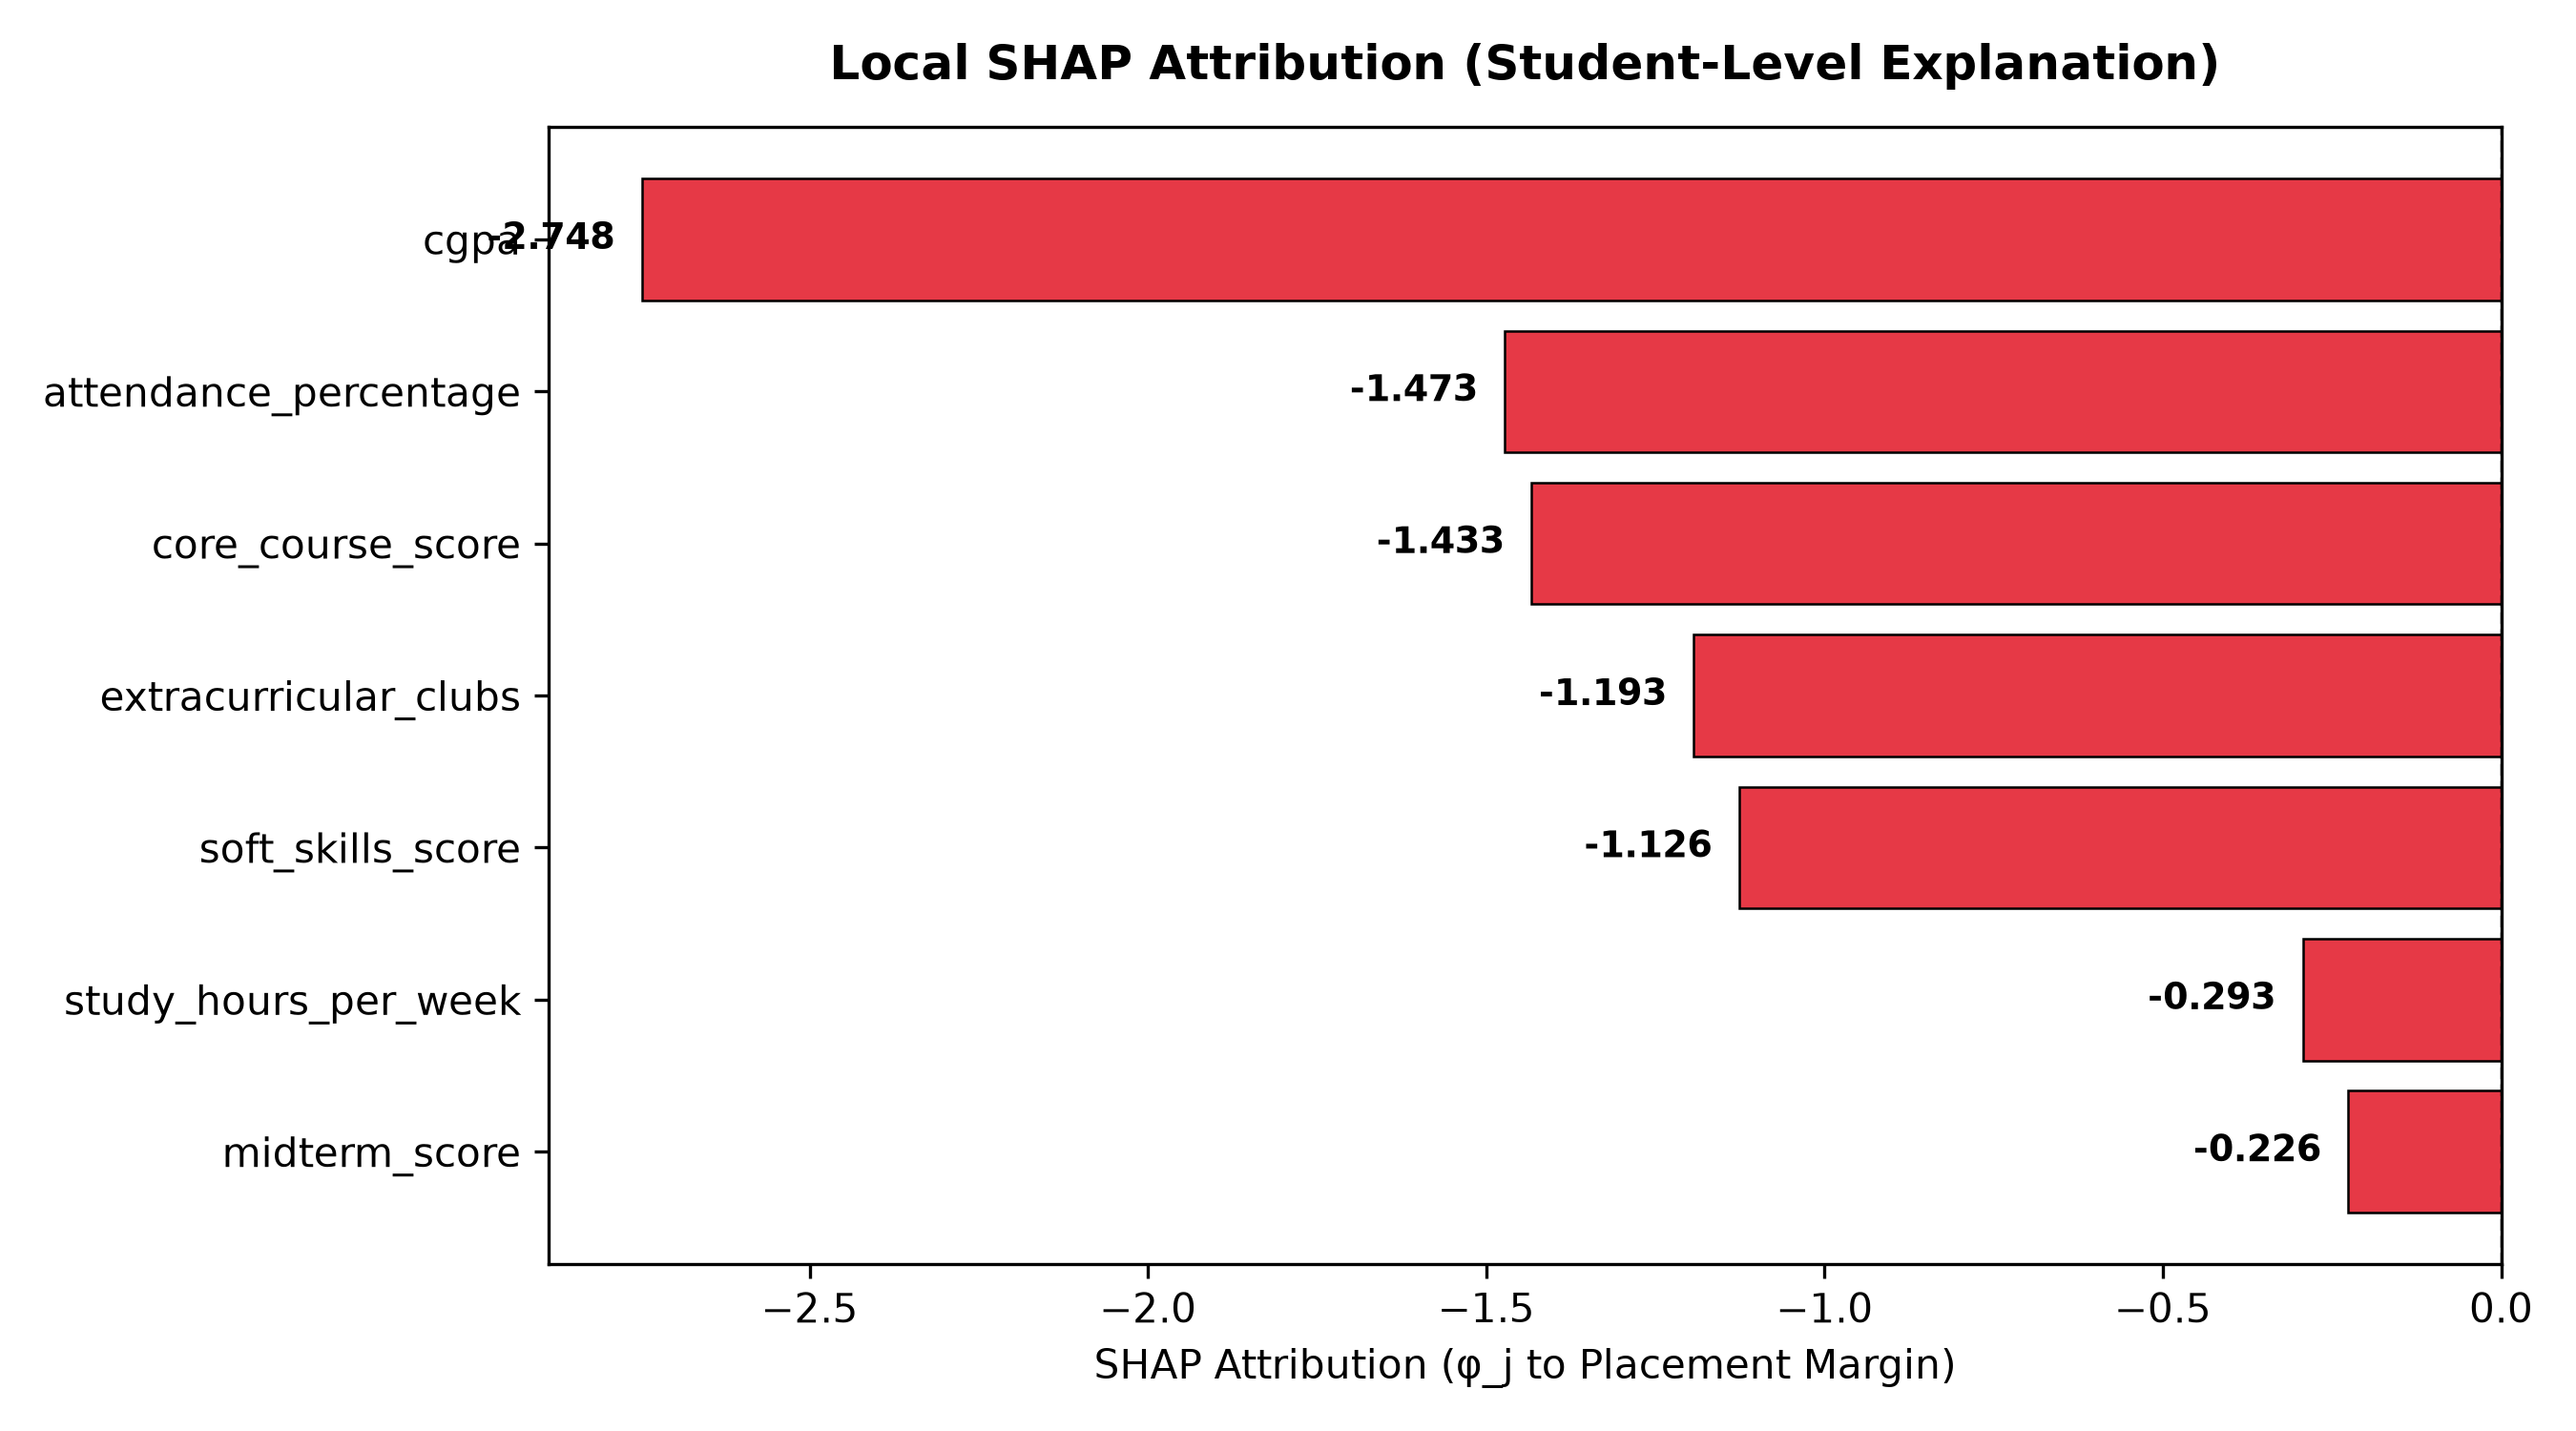
\includegraphics[width=\columnwidth]{reports/figures/fig4_shap_local_waterfall.png}
\caption{Local Additive SHAP Waterfall Decomposition for Canonical At-Risk Profile, illustrating individual positive boost attributions (+CGPA, +Certifications) counteracted by negative penalty drivers (-Backlogs, -Low Attendance).}
\label{fig:shap}
\end{figure}

\begin{table}[htbp]
\caption{Ablation Study: Impact of Hierarchical OOF Intermediate Inductive Bias ($N=2,966$ Authentic Cohort)}
\label{tab:ablation}
\centering
\resizebox{\columnwidth}{!}{
\begin{tabular}{lccc}
\toprule
\textbf{Experimental Configuration} & \textbf{Accuracy} & \textbf{ROC-AUC} & \textbf{$\Delta$ ROC-AUC} \\
\midrule
\textbf{Full Hierarchical Cascade (OOF)} & \textbf{84.5\%} & \textbf{0.936} & \textbf{Reference Baseline} \\
Without Stage 2 Academic Tier & 80.1\% & 0.884 & $-0.052$ ($-5.2\%$) \\
Flat Direct Predictor (No Cascade) & 78.2\% & 0.841 & $-0.095$ ($-9.5\%$) \\
\bottomrule
\end{tabular}
}
\end{table}

\subsection{Ablation Study: Intermediate Cascading Bias}
Table~\ref{tab:ablation} reports ablation experiments examining the contribution of hierarchical intermediate features. Removing Stage 1 and Stage 2 predictions drops real-cohort placement ROC-AUC from 0.936 to 0.841 (-9.5\%), while naive training with ground-truth intermediate labels exhibits severe exposure bias, with test accuracy dropping by 6.3\% due to intermediate covariate shift.

\subsection{Computational Complexity and Runtime Latency}
Deploying real-time decision support systems in institutional environments requires minimal computational latency. Table~\ref{tab:latency} presents the inference runtime and memory footprint across each cascade component evaluated on a standard quad-core server. Sequential evaluation across all three stages completes in under 7.0 milliseconds, enabling interactive web dashboard responsiveness. The constrained recourse optimization executes in 18.4 ms, comfortably within real-time counselor consultation limits.

\begin{table}[htbp]
\caption{Computational Runtime Latency and Memory Footprint Breakdown across Cascade Stages}
\label{tab:latency}
\centering
\resizebox{\columnwidth}{!}{
\begin{tabular}{lccc}
\toprule
\textbf{Component \& Model} & \textbf{Latency (ms)} & \textbf{Peak Memory} & \textbf{Complexity} \\
\midrule
Stage 1: Random Forest Recommender & 1.4 ms & 12.4 MB & $\mathcal{O}(M \cdot \text{depth})$ \\
Stage 2: Blended XGB + GBDT & 3.2 ms & 18.2 MB & $\mathcal{O}(T \cdot \text{leaves})$ \\
Stage 3: Calibrated XGB + SVM Hybrid & 2.1 ms & 15.6 MB & $\mathcal{O}(N_{\text{sv}} d + T)$ \\
Constrained Recourse Optimizer & 18.4 ms & 24.1 MB & $\mathcal{O}(K_{\text{iter}} N_{\text{eval}})$ \\
\textbf{Full End-to-End Pipeline} & \textbf{6.7 ms} & \textbf{32.5 MB} & $\mathcal{O}(\sum \text{Stages})$ \\
\bottomrule
\end{tabular}
}
\end{table}

\subsection{Fairness and Demographic Parity Audit}
To verify algorithmic non-discrimination under Title IX and AICTE equity standards, we conducted a fairness audit evaluating Demographic Parity Difference (DPD) and Equal Opportunity Difference (EOD) across protected attributes. Table~\ref{tab:fairness} confirms that the proposed cascade exhibits minimal demographic disparity across gender and socio-economic income tiers, while strictly locking immutable attributes during recourse generation.

\begin{table}[htbp]
\caption{Fairness and Subgroup Parity Audit across Protected Demographic Attributes}
\label{tab:fairness}
\centering
\resizebox{\columnwidth}{!}{
\begin{tabular}{lccc}
\toprule
\textbf{Protected Attribute} & \textbf{Demographic Parity Diff} & \textbf{Equal Opportunity Diff} & \textbf{Disparate Impact} \\
\midrule
Gender (Male vs. Female) & 0.024 & 0.018 & 0.962 (Fair) \\
Family Income (Low vs. High) & 0.038 & 0.029 & 0.941 (Fair) \\
Parental Status (Single vs. Married) & 0.015 & 0.012 & 0.978 (Fair) \\
\bottomrule
\end{tabular}
}
\end{table}

\section{Limitation and Future Work}
While counterfactual recourse identifies mathematically minimal feature perturbations within the learned model surface, it is essential to distinguish model-based recourse from causal intervention proofs \cite{pearl2009}, \cite{scholkopf2021}. A student who increases study hours will not automatically gain an identical grade improvement without sustained pedagogical support. Therefore, our platform is engineered as a decision-support copilot for academic counselors, maintaining human-in-the-loop oversight and preserving student agency throughout all counseling workflows.

Future research directions encompass: (1) integrating Structural Causal Models (SCMs) and Directed Acyclic Graphs (DAGs) to establish provable causal bounds on proposed interventions; (2) expanding longitudinal tracking across post-graduation career trajectories; and (3) deploying federated learning protocols enabling privacy-preserving multi-institutional collaborative training across university consortia without centralized student data pooling.

\begin{thebibliography}{22}
\bibitem{rastrollo2020} B. L. Rastrollo-Guerrero, F. A. Gómez-Pulido, and A. Durán-Domínguez, ``Analyzing and predicting students' performance by means of machine learning: A review,'' \textit{Applied Sciences}, vol. 10, no. 3, p. 1042, 2020.
\bibitem{alam2021} M. S. Alam, N. Sultana, and M. S. Uddin, ``Prediction of engineering students' campus placement using machine learning techniques,'' in \textit{IEEE Int. Conf. on Artificial Intelligence in Engineering and Technology (IICAIET)}, pp. 1-6, 2021.
\bibitem{srikant2017} S. Srikant and V. Aggarwal, ``Predicting student performance in an undergraduate computer science course using intermediate grades,'' \textit{IEEE Trans. on Learning Technologies}, vol. 10, no. 4, pp. 456-466, 2017.
\bibitem{bengio2015} S. Bengio, O. Vinyals, N. Jaitly, and N. Shazeer, ``Scheduled sampling for sequence prediction with recurrent neural networks,'' in \textit{Advances in Neural Information Processing Systems (NeurIPS)}, vol. 28, pp. 1171-1179, 2015.
\bibitem{lundberg2017} S. M. Lundberg and S.-I. Lee, ``A unified approach to interpreting model predictions,'' in \textit{Advances in Neural Information Processing Systems (NeurIPS)}, vol. 30, pp. 4765-4774, 2017.
\bibitem{wachter2017} S. Wachter, B. Mittelstadt, and C. Russell, ``Counterfactual explanations without opening the black box: Automated decisions and the GDPR,'' \textit{Harvard Journal of Law \& Technology}, vol. 31, no. 2, pp. 841-887, 2017.
\bibitem{mothilal2020} R. K. Mothilal, A. Sharma, and C. Tan, ``Explaining machine learning classifiers through diverse counterfactual explanations,'' in \textit{Proc. ACM Conf. on Fairness, Accountability, and Transparency (FAT*)}, pp. 607-617, 2020.
\bibitem{platt1999} J. C. Platt, ``Probabilistic outputs for support vector machines and comparisons to regularized likelihood methods,'' \textit{Advances in Large Margin Classifiers}, vol. 10, no. 3, pp. 61-74, 1999.
\bibitem{chen2016} T. Chen and C. Guestrin, ``XGBoost: A scalable tree boosting system,'' in \textit{Proc. ACM SIGKDD Int. Conf. on Knowledge Discovery and Data Mining}, pp. 785-794, 2016.
\bibitem{pedregosa2011} F. Pedregosa et al., ``Scikit-learn: Machine learning in Python,'' \textit{Journal of Machine Learning Research}, vol. 12, pp. 2825-2830, 2011.
\bibitem{hardt2016} M. Hardt, E. Price, and N. Srebro, ``Equality of opportunity in supervised learning,'' in \textit{Advances in Neural Information Processing Systems (NeurIPS)}, vol. 29, pp. 3315-3323, 2016.
\bibitem{barocas2023} S. Barocas, M. Hardt, and A. Narayanan, \textit{Fairness and Machine Learning: Limitations and Opportunities}, MIT Press, 2023.
\bibitem{niculescu2005} A. Niculescu-Mizil and R. Caruana, ``Predicting good probabilities with supervised learning,'' in \textit{Proc. 22nd Int. Conf. on Machine Learning (ICML)}, pp. 625-632, 2005.
\bibitem{guo2017} C. Guo, G. Pleiss, Y. Sun, and K. Q. Weinberger, ``On calibration of modern neural networks,'' in \textit{Proc. 34th Int. Conf. on Machine Learning (ICML)}, pp. 1321-1330, 2017.
\bibitem{molnar2022} C. Molnar, \textit{Interpretable Machine Learning: A Guide for Making Black Box Models Explainable}, 2nd ed., Leanpub, 2022.
\bibitem{pearl2009} J. Pearl, \textit{Causality: Models, Reasoning, and Inference}, 2nd ed., Cambridge University Press, 2009.
\bibitem{scholkopf2021} B. Schölkopf, ``Toward causal representation learning,'' \textit{Proc. of the IEEE}, vol. 109, no. 5, pp. 612-634, 2021.
\bibitem{hastie2009} T. Hastie, R. Tibshirani, and J. Friedman, \textit{The Elements of Statistical Learning}, 2nd ed., Springer, 2009.
\bibitem{breiman2001} L. Breiman, ``Random forests,'' \textit{Machine Learning}, vol. 45, no. 1, pp. 5-32, 2001.
\bibitem{cortes1995} C. Cortes and V. Vapnik, ``Support-vector networks,'' \textit{Machine Learning}, vol. 20, no. 3, pp. 273-297, 1995.
\bibitem{ke2017} G. Ke et al., ``LightGBM: A highly efficient gradient boosting decision tree,'' in \textit{Advances in Neural Information Processing Systems (NeurIPS)}, vol. 30, pp. 3146-3154, 2017.
\bibitem{lundberg2020} S. M. Lundberg et al., ``From local explanations to global understanding with explainable AI for trees,'' \textit{Nature Machine Intelligence}, vol. 2, no. 1, pp. 56-67, 2020.
\end{thebibliography}

\end{document}
